\section{Classification and placement}
\label{sec:intro:virt_and_cont}
The architectural difference of full virtualization and containerization concept is shortly classified in this segment.

Containerization is widely used in cloud environments. Containers are almost the foundation of every cloud environment.
However classical virtualization exists long before container technologies.
Both concepts have advantages and disadvantages. 
This is the reason why they are also combined as hybrid concepts \cite{6498558}.
Figure \ref{fig:intro:diff_container_vm} was created in \cite{evol_cont} and shows the architectural difference between container technology and full virtualization.
 
\begin{figure}[htbp]
 \centering
 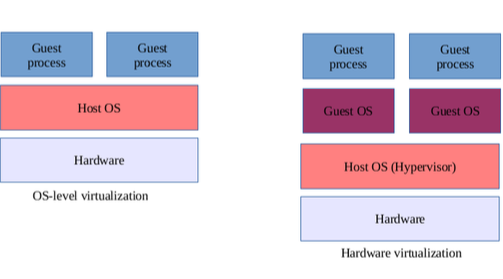
\includegraphics[width=0.7\textwidth]{gfx/examples/os_virt_diff}
 \caption{Architectural difference container and full virtualization}
 \label{fig:intro:diff_container_vm}
\end{figure}
Full virtualization allows it to run an entire guest operating system in a virtual machine (VM) on a host operating system. 
This is possible through an installed piece of software called hypervisor which is built classically on top of the originally operating system. 
This virtualization model provides solid security through this additional isolation layer. 
One obvious drawback is the heavyweight and high resource usage characteristic.
In contrast to classical virtualization a container does not need an additional operating system layer as seen in Figure \ref{fig:intro:diff_container_vm}. 
The container is just using and sharing the underlying kernel from the host. 

Containerization technology is closer to the underlying host operating system than the classical virtualization strategy. 
That makes containers more lightweight and flexible. 
Comparisons between container concepts and classical virtualization with regard to the application purposes are described in \cite{7921010}
The next section offers a closer look at containerization paradigm itself.

